\subsection{Ajuste de Brilho}

Ajuste de brilho por correção gama. A implementação é feita convertendo a imagem para uma matriz $A$ com valores em [0, 1]. Com isso, é feita a transformação $B = A^{\frac{1}{\gamma}}$,
sendo $B$ convertida para uma imagem com valores em [0, 255] novamente.

O fator $\gamma$ é passado como argumento para o comando \text{aj.brilho}. Por exemplo, a \cref{fig:ajbrilho} foi feita com o sequinte comando:

\begin{minted}{bash}
    $ python main.py imagens/color.png -o out.png aj.brilho 2.5
\end{minted}

\begin{figure}[H]
    \centering
    \begin{subfigure}{0.45\textwidth}
        \centering
        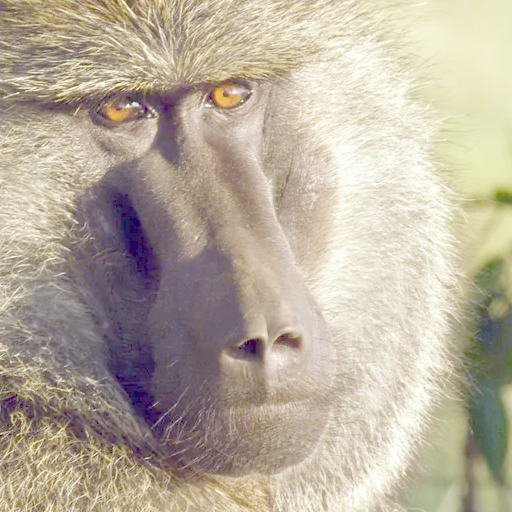
\includegraphics[width=6cm]{resultados/colorgama.png}
        \caption{\texttt{imagens/color.png}}
        \label{fig:ajbrilho}
    \end{subfigure}%
    \begin{subfigure}{0.45\textwidth}
        \centering
        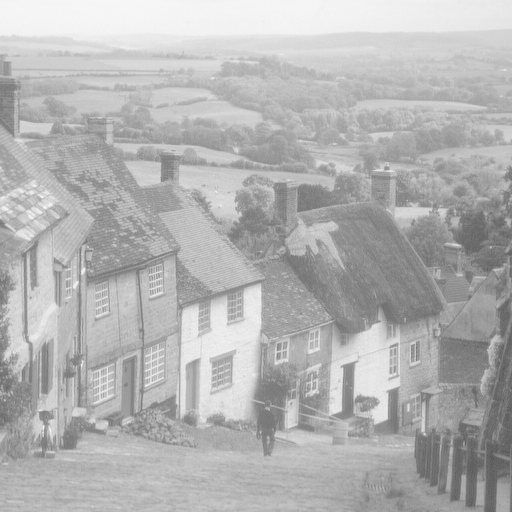
\includegraphics[width=6cm]{resultados/citygama.png}
        \caption{\texttt{imagens/city.png}}
    \end{subfigure}

    \caption{Brilho ajustado com $\gamma = 2.5$.}
\end{figure}

\begin{listing}[H]
    \caption{Comando \texttt{aj.brilho GAMA}}

    \begin{minted}{python}
        def ajuste_brilho(imagem, gama):
            A = imagem / 255
            B = A ** (1 / gama)
            return (B * 255).astype(np.uint8)
    \end{minted}
\end{listing}
